%TCIDATA{Version=5.00.0.2606}
%TCIDATA{LaTeXparent=0,0,..\Elvira-Book.tex}

%TCIDATA{ChildDefaults=chapter:1,page:1}


\section{Algorithms of evaluation of IDs}

The objective of the evaluation of an ID is to obtain a decision table for
each decision node, containing the policy for that decision (see SECTION
1.1.3). So, it is necessary to evaluate the ID with specific algorithms.
Elvira have implemented several algorithms of evaluation of IDs. Now, we are
going to describe the algorithms available in Elvira to obtain an exact
evaluation, an approximate solution or simply a qualitative evaluation of
the ID.

\subsection{Exact algorithms}

Exact algorithms let us have an exact evaluation of the ID. This implies
that there is no error in the values that compose the decision tables
returned by the exact algorithm, so that the decision maker is certain of
the policies obtained. First, we expose the basic algorithms of evaluation
for influence diagrams. Next, we present a new kind of influence diagram
which take advantage of the separable utility functions and we describe
their algorithms algorithms.

\subsubsection{Exact algorithms for influence diagrams}

The basic exact algorithms for the evaluation of IDs are arc-reversal \cite%
{shachter86} and variable elimination \cite{jensen01}.

\paragraph{Arc-reversal algorithm}

The arc-reversal algorithm \cite{shachter86} was the first algorithm of
evaluation of IDs that did not require an auxiliary structure to solve the
decision problem. It takes advantage of the basis of the dynamic programming
and of the calculus of probabilities in Bayesian networks.

The algorithm assumes that the ID is oriented (it has got an only utility
node) and the decision nodes are ordered. This second condition is kept if
there is a path in the ID that contains to all the decision nodes.

The ID is transformed during the evaluation, but its optimal policies remain
unchanged. These transformations modify the probability potentials of the
chance nodes and the utility potential of the utility node and compute the
decision tables. There are three basic transformations in the arc-reversal
algorithm.

\begin{itemize}
\item \texttt{Elimination of a chance node. }It modifies the utility
potential by averaging it with the probability potential of the node to
eliminate.

\item \texttt{Elimination of a decision node. }It modifies the utility
potential through maximization by selecting the alternative of the decision
that maximizes the expected utility.

\item \texttt{Arc reversal. }It changes the direction of an arc in the ID by
applying Bayes theorem.
\end{itemize}

When a node is eliminated it is deleted from the ID. It can makes other
nodes become barren, i.e., nodes without successors. Barren nodes can be
deleted directly from the ID because the do not influence the decision table
of any decision.

The pseudo code for the arc-reversal algorithm is as follows.

\noindent \textsf{\textbf{ALGORITHM Arc reversal($ID$)}}

\bigskip \noindent INPUT: An ID with utility node $U$.

\noindent OUTPUT: A set of decision tables that maximize the expected
utility.

\begin{enumerate}
\item Initial phase

\begin{enumerate}
\item Verify that the ID is oriented and the decisions are ordered

\item Eliminate redundancy and barren nodes from the ID
\end{enumerate}

\item WHILE $parents(U)\neq \emptyset $ DO

\begin{itemize}
\item IF there exists a node $C\in V_{C}$ such that $children(C)=\{U\}$ THEN
remove chance node $C$

\item ELSE IF there exists a node $D\in V_{D}$ such that $children(D)=\{U\}$
$and$ $parents(U)\subseteq parents(D)\cup \{D\}$ THEN remove decision $D$
and remove barren nodes

\item ELSE find a $C\in V_{C}$ such that $C\in parents(U)$ $and$ $%
children(C)\cap V_{D}=\emptyset ,$ reverse the arcs from $parents(C)$ to $C$
and remove chance node $C$
\end{itemize}
\end{enumerate}

\paragraph{Variable elimination algorithm.}

This method let us evaluate an ID when the decisions are ordered. Also, it
allows to have several utility nodes without successors, existing an
implicit sum among them.

The algorithm constructs initially a order among the decisions: $%
D_{1},...,D_{n}.$ It uses this order of decisions to partition $V_{C}$
according to when the chance nodes are observed. So, $I_{0}$ is the set of
chance nodes observed before $D_{1}$ ($I_{0}=infPred(D_{1})$)$.$ $I_{i}$ is
the set of chance nodes observed after $D_{i}$ but before $D_{i+1}$ ($%
I_{i}=infPred(D_{i+1})\setminus I_{i-1}$). $I_{n}$ are the chance observed
after the last decision $D_{n}$. So, there exists partial order among the
nodes: {\normalsize $I_{0}<D_{1}<\ldots <D_{n}<I_{n}.$}

The variable elimination algorithm eliminates sequentially the variables
from the ID according to this partial order. So, it eliminates the chance
nodes in $I_{n}$ by sum-marginalization, then max-marginalize $D_{n}$,
sum-marginalize $I_{n-1},$ and so on. Because sum-marginalization commute,
the nodes in each $I_{i}$ can be eliminated in any arbitrary order, so there
can be several total orders compatible with the partial order of the ID. The
total order in which the variables are eliminated can be set set initially
or after each variable is eliminated. The procedure presented here sets the
total order initially. The algorithm for eliminating a variable and the
variable elimination algorithm that evaluates the ID are as follow.

\noindent \textsf{\textbf{ALGORITHM EliminateVariable(}}$\Phi ,\Psi ,X$%
\textsf{\textbf{)}}

\bigskip \noindent INPUT: A set of probability potentials $\Phi ,$ a set of
utility potentials $\Psi $ and a variable $X$ to eliminate

\noindent OUTPUT: The sets of potentials $\Phi $ and $\Psi $ after
eliminating the variable $X$

\begin{enumerate}
\item Let $\Phi _{X}$ all potentials in $\Phi $ with $X$ in their domains

\item Let $\Psi _{X}$ all potentials in $\Psi $ with $X$ in their domains

\item IF $X$ is a chance variable THEN

\begin{itemize}
\item $\phi ^{-X}=\sum_{X}\prod \Phi _{X}$

\item $\psi ^{-X}=\sum_{X}\prod \Phi _{X}\left( \sum \Psi _{X}\right) $
\end{itemize}

\item IF $X$ is a decision variable THEN

\begin{itemize}
\item $\phi ^{-X}=\max_{X}\prod \Phi _{X}$

\item $\psi ^{-X}=\max_{X}\prod \Phi _{X}\left( \sum \Psi _{X}\right) $
\end{itemize}

\item Update to $\Phi $ and $\Psi $

\begin{itemize}
\item $\Phi =\left( \Phi \setminus \Phi _{X}\right) \cup \{\phi ^{-X}\}$

\item $\Psi =\left( \Psi \setminus \Psi _{X}\right) \cup \{\psi ^{-X}/\phi
^{-X}\}$
\end{itemize}
\end{enumerate}

\noindent \textsf{\textbf{ALGORITHM VariableElimination(}ID\textbf{)}}

\bigskip \noindent INPUT: An ID with set of probability potentials $\Phi $
and set of utility potentials $\Psi $

\noindent OUTPUT: A set of decision tables that maximize the expected
utility.

\begin{enumerate}
\item Construct a total ordering of the variables from the partial order
induced by the ID

\item WHILE there are variables to eliminate{\normalsize \ }DO

\begin{enumerate}
\item Let $X$ the next variable to eliminate according to the total ordering

\item \textsf{\textbf{EliminateVariable(}}$\Phi ,\Psi ,X$\textsf{\textbf{)}}
\end{enumerate}
\end{enumerate}

\subsubsection{Exact algorithms for ID with super-value nodes}

The variable elimination algorithm presents an important advantage over the
arc-reversal algorithm because it let us have an additive (or
multiplicative) decomposition of the utility function. However, it cannot
evaluate an ID whose utility function can have arbitrarily nested sums and
products. Several algorithms have been developed to take advantage of the
separability of the utility functions: Tatman and Shachter's algorithm \cite%
{tatman90} and variable elimination for IDs with super-value nodes \cite%
{luque04}. Next, the super-value nodes are introduced in the influence
diagram formalism and we expose the two algorithms of evaluation.

\paragraph{IDs with super-value nodes}

In the influence diagram of the reactor problem (see Figure \ref{reactorID})
the preferences of the decision maker were represented with a function (see
Figure \ref{prefTree}). However, according to how the preferences were
defined, the function of preferences is separable, which means we can
represent it as the sum of three functions. These functions can be displayed
in Figure \ref{prefTreeSV}, where the trees represent respectively the
profits due to the conventional reactor and the advanced reactor and the
cost of the test. These three functions depend on less variables that the
original function, which will let us apply during the evaluation the
operators of sum-marginalization and max-marginalization to some components
of the utility function instead of the whole function.

\begin{figure}[h]
\begin{center}
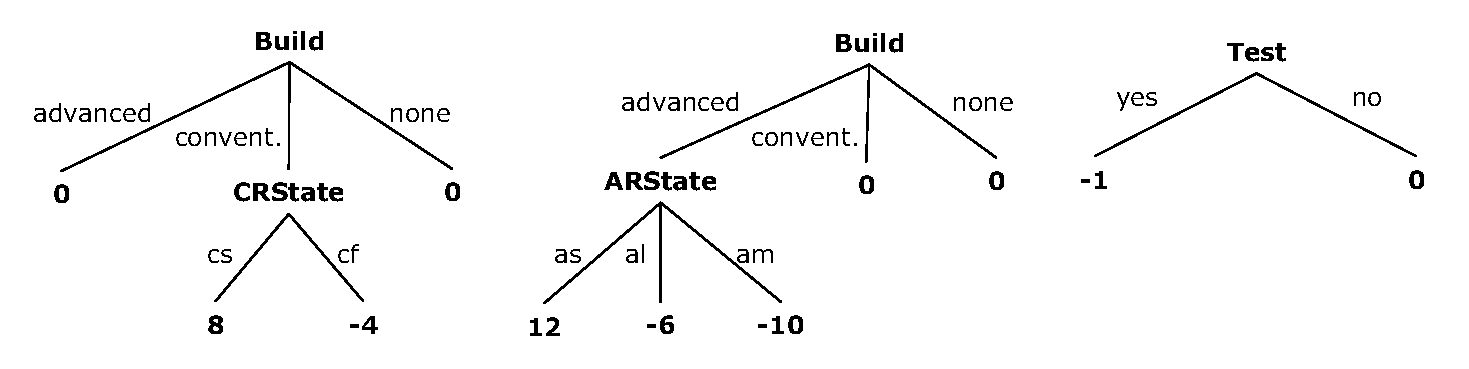
\includegraphics[scale=0.5]{./ID/fig/prefTreeSV} \vspace{-0.5cm}
\end{center}
\caption{Additive decomposition of the preferences for reactor build problem}
\label{prefTreeSV}
\end{figure}

A new kind of utility node was introduced by \cite{tatman90} in the
influence diagram formalism to represent these separable functions.
This new kind of node was called super-value node, and let us
represent the sum or the product of other utility nodes. So, Figure
\ref{reactorIDSV} represents the reactor problem with an ID with a
super-value node. This node is a sum node and their parents are
utility nodes that represent the three functions exposed in the
trees of Figure \ref{prefTreeSV}.

\begin{figure}[h]
\begin{center}
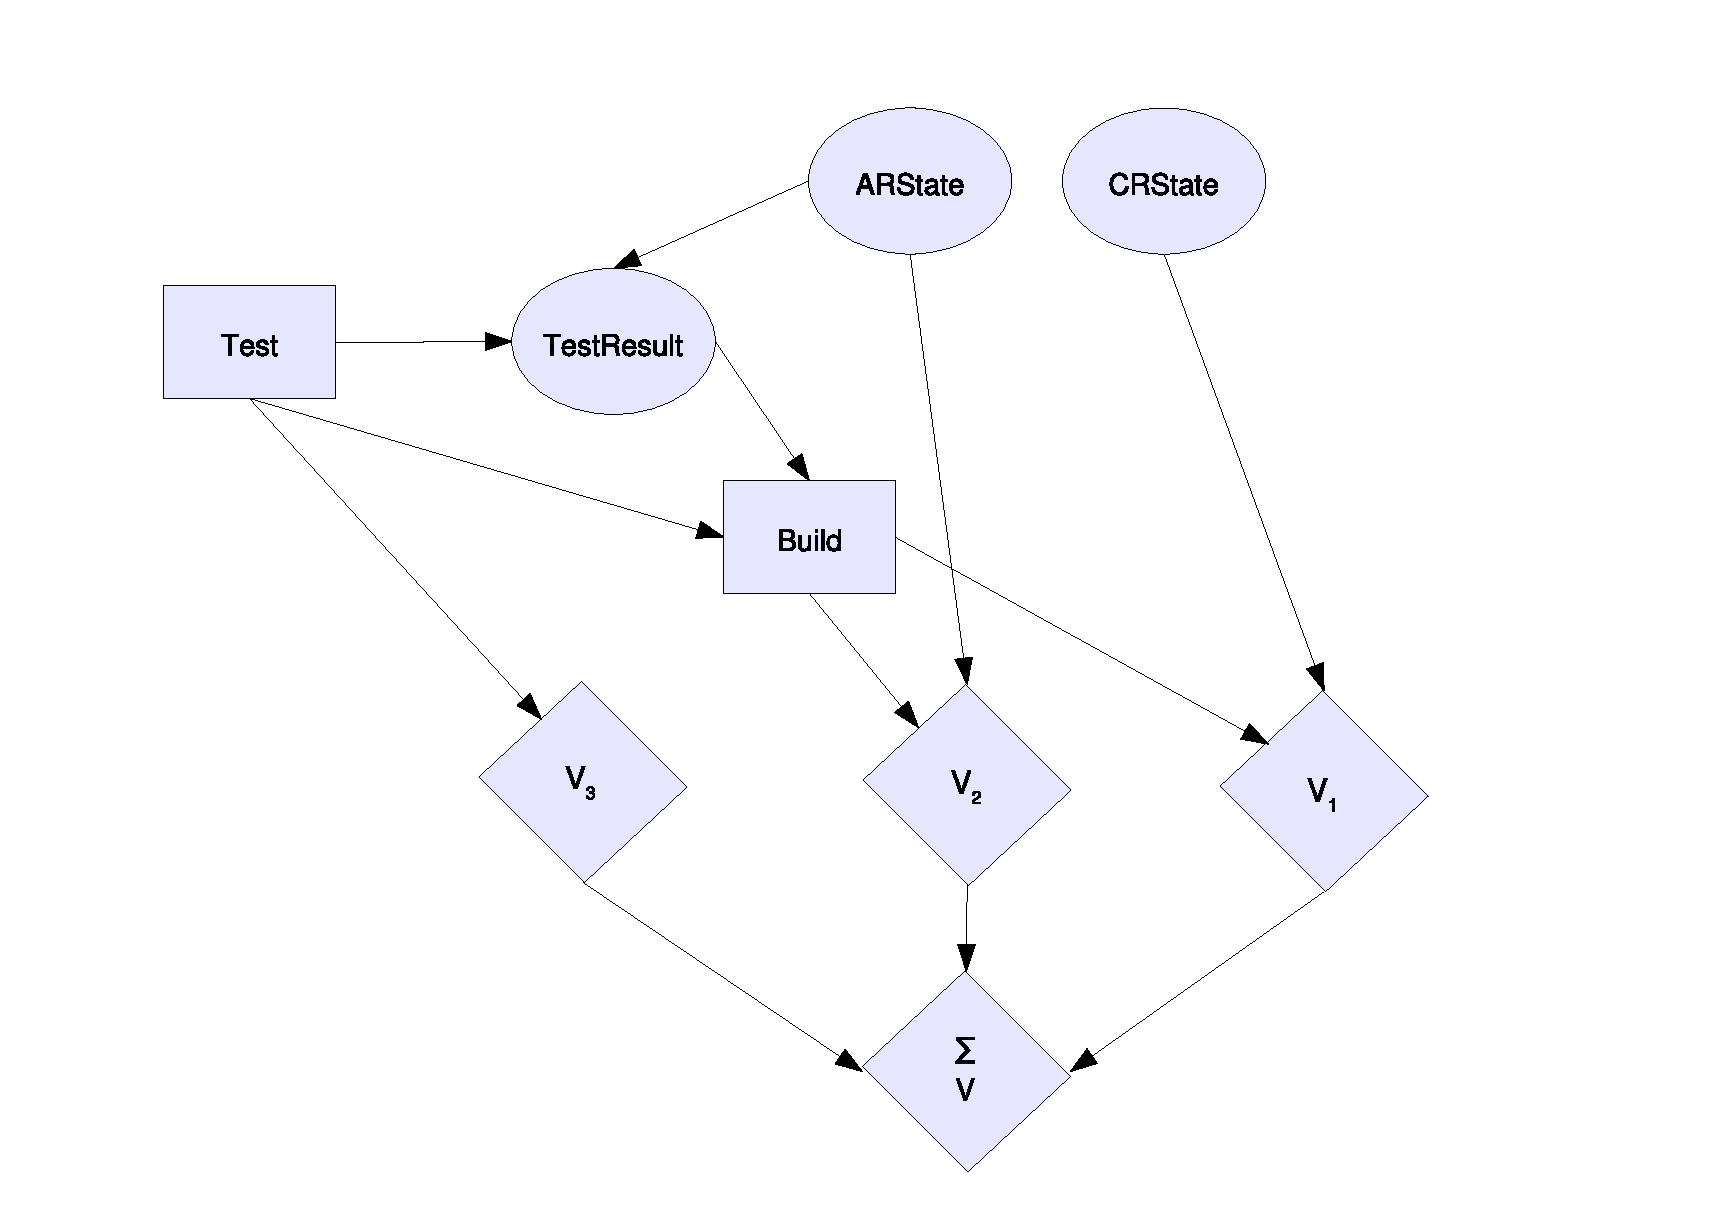
\includegraphics[scale=0.4]{./ID/fig/reactorIDSV} \vspace{-0.5cm}
\end{center}
\caption{Reactor influence diagram with a super-value node}
\label{reactorIDSV}
\end{figure}

\paragraph{Tatman and Shachter's algorithm}

\cite{tatman90} proposed the first algorithm to evaluate IDs with
super-value nodes. They use the basic scheme of the arc reversal
algorithm for traditional IDs, but adapted to cope with super-value
nodes. The authors try to keep the separability as long as possible
during the evaluation.

The conditions that have to take place for eliminating a chance or decision
node are modified because of the presence of super-value nodes. This can
make the algorithm merges several utility nodes into an only utility node to
allow us to perform the elimination operation. Then, one basic
transformation is added to the three basic transformations of the
arc-reversal algorithm, which we describe as follow.

\begin{itemize}
\item \texttt{Merging of utility nodes. }It merges several utility nodes
which are parents of the same super-value node into a new super-value node.
\end{itemize}

As an example of this operation, look to the ID with super-value nodes of
Figure \ref{reactorIDSV}. The utility nodes $v_{1}$ and $v_{2}$ are parents
of the sum node $v$. We can merge $v_{1}$ and $v_{2}$ into a new utility
node $v_{4}.$ This node would join the functions of preferences of $v_{1}$
and $v_{2}$, so that it would depend on the variables $Build,$ $ARState$ and
$CRState.$ After the merging the sum node $v$ would have only two parents, $%
v_{3}$ and $v_{4},$ while $v_{1}$ and $v_{2}$ would disappear from the ID.
Now we are going to see how these merging of utility nodes can be necessary
to eliminate chance or decision nodes.

The algorithm assumes that the ID with super-value nodes is oriented: each
utility node is parent of an only utility node, except one that have no
children and is called terminal utility node. Also, the decision nodes must
be ordered.

Also, Tatman and Shachter proposed an heuristic to reduce the storage size
of the structure of utility nodes during the evaluation. This heuristic was
called the \textit{subset rule}. The authors explained that if two utility
nodes $r_{1}$ and $r_{2}$ have the same successor, a super-value node $r$,
and $pa(r_{1})\subseteq pa(r_{2}),$ then removing $r_{1}$ and $r_{2}$
(possibly merging $r_{1}$ and $r_{2}$ into a new value node $r^{\prime }$ if
they are not the only predecessors of $r$), will not increase the size of
any operation necessary to solve the ID and so they should be merged.

It is necessary to define an additional term specific of IDs with
super-value nodes to understand Tatman and Shachter's algorithm. \ A node $X$
is said to be a \textit{functional predecessor} of an utility node $U$ if
the function associated with node $U$ can be written as a deterministic
function for which $X$ is an argument. So, every utility $V\in $ $ant(U)$ is
a functional predecessor of $U.$ Also, if $X$ is a chance or decision node,
then $X$ is a functional predecessor of $U$ if $X$ is parent of $U$ or some
utility node functional predecessor of $U.$ The set of functional
predecessors of a node $U$ is denoted as $funcPred(U).$ Also, we use $%
funcPred_{C\cup D}(U)$ to denote the set of chance and decision nodes that
are functional predecessors of $U.$ For example, for the ID with super-value
nodes of Figure \ref{reactorIDSV}, $funcPred(V_{1})=funcPred_{C\cup
D}(V_{1})=\{Build,$ $CRState\}$ whereas $funcPred(V)=%
\{V_{1},V_{2},V_{3},Test,Build,ARState,CRState\}$ and $funcPred_{C\cup
D}(V)=\{Test,Build,ARState,CRState\}.$

The basic procedure of Tatman and Shachter's algorithm can be presented with
a scheme very similar to the arc-reversal algorithm.

\textsf{\textbf{ALGORITHM Tatman and Shachter's($ID$)}}

\bigskip \noindent INPUT: An ID with super-value nodes with terminal utility
node $U_{0}$.

\noindent OUTPUT: A set of decision tables that maximize the expected
utility.

\begin{enumerate}
\item Initial phase

\begin{enumerate}
\item Verify that the ID is oriented and the decisions are ordered

\item Eliminate barren nodes from the ID
\end{enumerate}

\item WHILE $parents(U_{0})\neq \emptyset $ DO

\begin{itemize}
\item IF the subset rule holds for any set of utility nodes THEN merge these
utility nodes (possibly adding a sum or a product node)

\item IF there exists a node $C\in V_{C}$ such that $children(C)\subseteq
V_{U}$ THEN

\begin{itemize}
\item DO merge utility nodes UNTIL $card(children(C))=1$

\item remove chance node $C$
\end{itemize}

\item ELSE IF there exists a node $D\in V_{D}$ that verifies these three
conditions: a) $children(D)\subseteq V_{U},$ b) there exists a utility node $%
S$ such that $funcPred_{C\cup D}(S)\subseteq $ $parents(D)\cup \{D\}$ and c)
all directed paths from $D$ to $U_{0}$ contain $S$ THEN

\begin{itemize}
\item merge all utility nodes ancestors of $S$

\item remove decision $D$ and remove barren nodes
\end{itemize}

\item ELSE find a $C\in V_{C}$ such that $C\in funcPred(U_{0})$ and $%
children(C)\cap V_{D}=\emptyset ,$ reverse the arcs from $parents(C)$ to $C$
and remove chance node $C$
\end{itemize}
\end{enumerate}

\paragraph{Variable elimination for IDs with super value nodes algorithm.}

\cite{luque04} proposed an algorithm based in variable-elimination
algorithm in order to evaluate IDs with super-value nodes. The
objective of the proposed algorithm was to overcome two shortcomings
of Tatman and Shachter's algorithm: a) it requires dividing
potentials when reversing arcs, and b) it sometimes merge too much
early utility nodes, which can introduce redundant variables in the
policies.

We are going to present the basic algorithm of variable elimination for IDs
with super-value nodes. Next, we will present some variations of this
algorithm.

\subparagraph{Basic algorithm of variable elimination for IDs with
super-value nodes}

The basic algorithm of variable-elimination for IDs with super-value nodes
(VESV) represents the sets of probability and utility potentials of an ID as
a tree of potentials (ToP), whose leaves (terminal nodes) represent
potentials, and non-terminal nodes represent either the sum or the product
of the potentials represented by their children. So, there

Then, the next expression is called the \textit{matrix} of the ID: $\left(
\prod_{i}p(X_{i}|pa(X_{i}))\right) \psi _{0},$ where $\psi _{0}$ is the
utility function of the terminal utility node $U_{0}$ and $X_{i}$ are the
different chance variables of the ID. The variable elimination for ID with
super-value nodes algorithm constructs a ToP which represents the matrix of
an ID. The subsequent eliminations of variables will be performed over the
ToPP.

For example, consider us the ID with super-value nodes of the reactor
problem (see Figure \ref{reactorIDSV}). Its matrix is given by the
expression $P(ARState)\cdot P(CRState)\cdot P(TestResult|Test,ARState)\cdot
(U_{1}(Build,CRState)+U_{2}(Build,ARState)+U_{3}(Test)),$ which from the
ToPP of Figure \ref{fig:ToPreactorIDSV} is constructed directly.

\begin{figure}[h]
\begin{center}
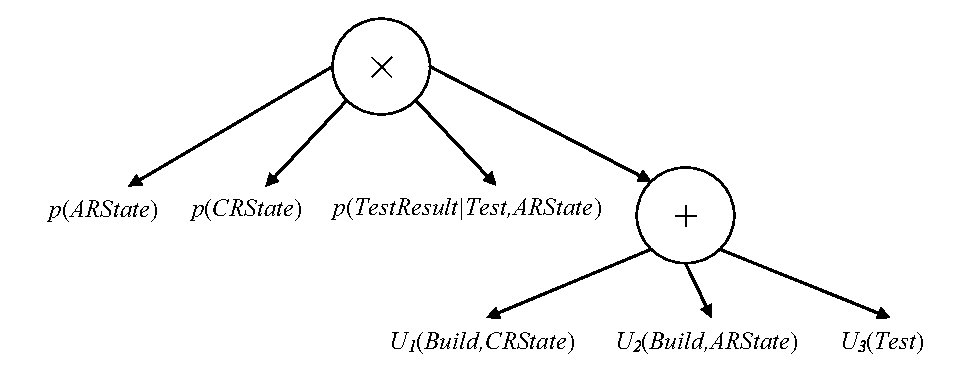
\includegraphics[scale=0.6]{./ID/fig/ToPreactorIDSV} \vspace{-0.5cm}
\end{center}
\caption{ToP of the reactor ID with super-value nodes}
\label{fig:ToPreactorIDSV}
\end{figure}
\bigskip

We are going to define several equivalence transformations on the ToP
necessary to understand the algorithm VESV.

\begin{itemize}
\item \texttt{Elimination of redundant nodes. }A non-terminal node of a ToP
is redundant if it is of the same type as its parent or if it only has one
child. Redundant nodes are removed transferring its children to its parent.

\item \texttt{Compaction of leaves. }We can operate several leaves children
of the same operator. For example, we could compact the leaves $P(ARState)$
and $P(TestResult|Test,ARState)$ of figure, so that we would obtain the ToPP
of Figure \ref{fig:compactedToPreactorIDSV}.

\item \texttt{Reduction of non-terminal nodes. }Reducing a non-terminal node
consists in transform it in an only leaf by compacting all the leaves of its
subtree and by eliminating all redundant nodes. For example, the sum node of
Figure \ could be reduced, so its subtree would be substituted by the leaf $%
U_{1}(Build,CRState)+U_{2}(Build,ARState)+U_{3}(Test).$

\item \texttt{Application of distributive property. }The distributive
property can be applied on a ToP. For example, in Figure \ref%
{fig:distributionToP}.a we have that $n_{1}$ is a sum node. We can
distribute $n_{2}$ with respect to $n_{1}$, obtaining the ToP of Figure \ref%
{fig:distributionToP}.b. Note that $n_{2}$ could be a leaf or a non-terminal
node root of a subtree.
\end{itemize}

\begin{figure}[h]
\begin{center}
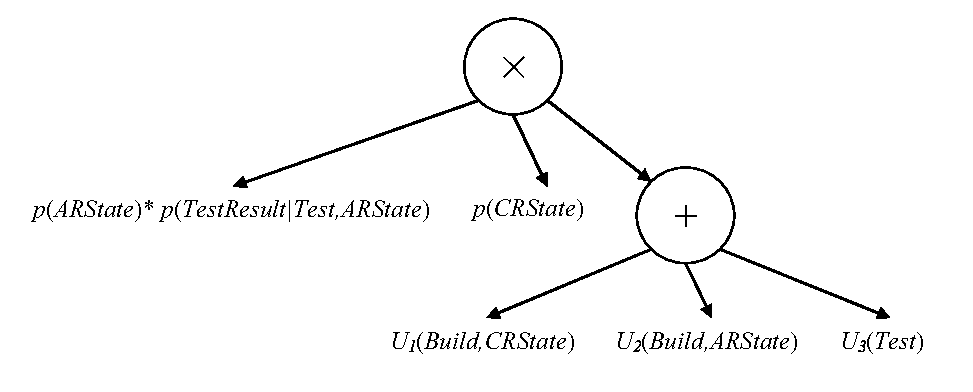
\includegraphics[scale=0.6]{./ID/fig/compactedToPreactorIDSV} \vspace{-0.5cm}
\end{center}
\caption{ToP equivalent to Figure \ref{fig:ToPreactorIDSV}, where
the leaves $P(ARState)$ and $P(TestResult|Test,ARState)$ have been
compacted} \label{fig:compactedToPreactorIDSV}
\end{figure}

\begin{figure}[tbp]
\centering
\begin{tabular}{cc}
{%
\parbox[b]{1.6621in}{\begin{center}
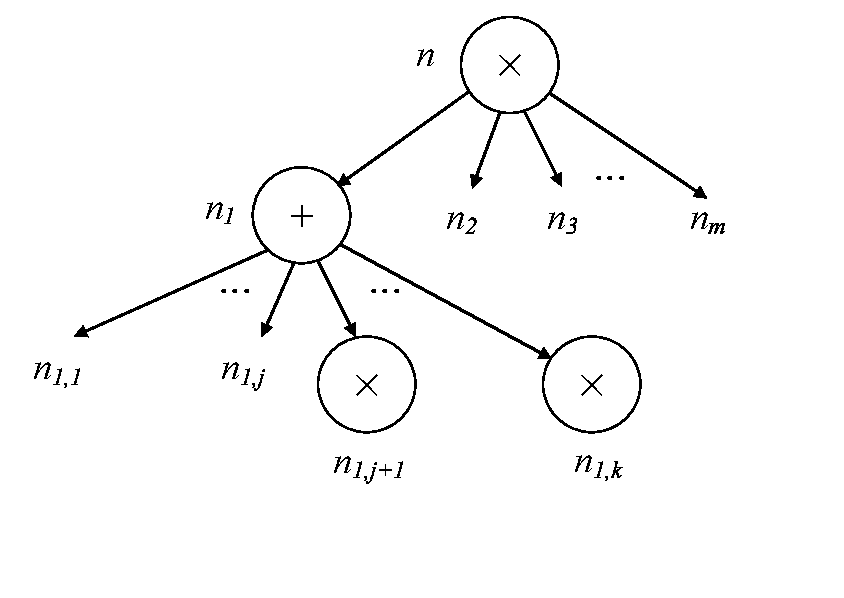
\includegraphics[
scale=0.4
]{./ID/fig/beforeDistributionToP.eps}\\
Fig. (a)
\end{center}}} & {%
\parbox[b]{2.9165in}{\begin{center}
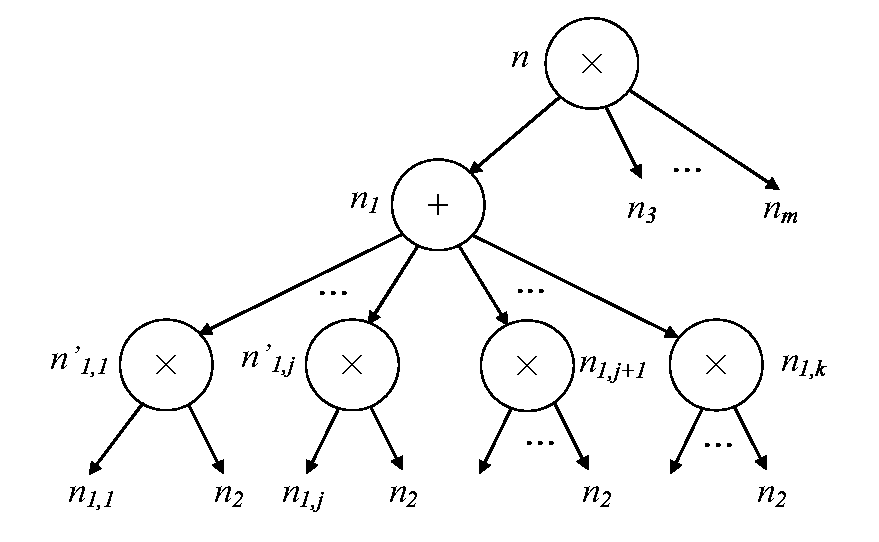
\includegraphics[
scale=0.4
]{./ID/fig/afterDistributionToP.eps}\\
Fig. (b)
\end{center}}}%
\end{tabular}%
\caption{The ToP (b)\ is equivalent to (a), in which $n_{2}$ has been
distributed with respect to $n_{1}$.}
\label{fig:distributionToP}
\end{figure}

We must define the concept of \textit{forked, }which is crucial when
the algorithm VESV eliminating a chance variable. A product node of
the ToP is said to be \textit{forked} with respect to a variable $A$
if $A$ appears in more than one of the subtrees children of the ToP.
For example, the root of the ToP of Figure \ref{fig:ToPreactorIDSV}
is forked with respect to $A$ because $A$ appears in two children of
the root: the leaf $P(CRState)$ and the subtree
$(U_{1}(Build,CRState)+U_{2}(Build,ARState)+U_{3}(Test)).$

As in variable-elimination algorithm for traditional IDs, the algorithm of
variable elimination for IDs with super-value nodes (VESV) assumes that
there exists a partial order among the nodes: {\normalsize $%
I_{0}<D_{1}<\ldots <D_{n}<I_{n}.$ }The variables are eliminated of the ToP
according to a total order compatible with the partial order. Now, we can
understand the most of the steps of the algorithm VESV, whose main
differences with respect to the variable-elimination algorithm for
traditional IDs are about how chance and decision variables are eliminated
of the ToP.

\noindent \textsf{\textbf{ALGORITHM VariableEliminationSV(}ID\textbf{)}}

\bigskip \noindent INPUT: An ID with super-value nodes

\noindent OUTPUT: A set of decision tables that maximize the expected
utility.

\begin{enumerate}
\item Construct a total ordering of the variables from the partial order
induced by the ID

\item Construct the ToP and remove the redundant nodes

\item WHILE there are variables to eliminate{\normalsize \ }DO

\begin{enumerate}
\item Let $X$ the next variable to eliminate according to the total ordering

\item IF $X$ is a chance variable

\begin{enumerate}
\item Convert all forked (product) nodes with respect to $X$ to non-forked
by doing a depth-first search in the ToP

\item Sum-marginalize $X$ out of the leaves which depend on $X$
\end{enumerate}

\item IF $X$ is a decision variable

\begin{enumerate}
\item Look for the smaller subtree that includes all appearances of $X$

\item Reduce that subtree and maximize it over $X$
\end{enumerate}
\end{enumerate}
\end{enumerate}

When the ToP has no forked (product) nodes to apply the operator
$\sum_{A}$ to the ToP is equivalent to apply it to their leaves
dependent on $A$ (see details in \cite{luque04}). Forked nodes are
converted to non-forked by compacting the leaves dependent on $X$
and by applying the distributive property until all nodes are
unforked. The depth-first search of forked nodes in the ToP
guarantees certain computations of potentials will not be repeated.

\subparagraph{Variations of the algorithm VESV}

Some modifications to the basic algorithm VESV can be performed.

The first modification consists in to use an acyclic directed graph of
potentials (ADGoP) instead of a tree of potentials. This makes we obtain
savings in computational size and storage size. Also, using an ADGoP makes
we cope with IDs whose utility nodes may have several children, which was
not tackled by Tatman and Shachter's algorithm.

Furthermore, other important modification is about taking advantage of the
unity-potentials. These are computations that results in a potential equal
to 1 which does not depend on any variable. Some of these computations are $%
\sum_{H}p(H|T)$ and $\sum_{A}[\phi _{A}/\sum_{A}\phi _{A}].$ They are very
frequent in the calculation of probabilities in Bayesian networks and in
variable-elimination algorithms, so detecting unity-potentials brings about
important computational savings.

Other variation of the basic algorithm includes the possibility of
performing divisions. The algorithm VESV with divisions (VESVD) operates
similarly to the algorithm VESV, but it handles separately the probability
and utility potentials through a ToPP and an ADGoP respectively. The use of
divisions makes the algorithm a bit less time-efficient. However, it let us
compute not only the optimal policies but their utilities. Furthermore, the
algorithm VESVD can return policies with less required variables than VESV.

Finally, the subset rule of Tatman and Shachter's algorithm can be adapted
to the algorithm VESV. So, when two leaves with potentials $\phi _{1}$ and $%
\phi _{2}$, have the same parent, an operator node, and $dom(\phi
_{1})\subseteq dom(\phi _{2}),$ then compacting those two leaves will not
increase the storage size during the evaluation of the ID.

\input ID/AproxEvaluation
